%! TEX root = ./original_dyck_area.tex
\documentclass[12pt]{article}

%--------Packages-------------
\usepackage[noquiver]{kyrem1sty}
%----------------------------


%--------Bibliography---------
\usepackage[backend=biber,style=alphabetic,doi=false,isbn=false,url=false,eprint=false]{biblatex}
\addbibresource{/home/kyrem1/Mathematics/bibs/comborefs.bib}
%----------------------------


%--------Hyper Setup-------
\hypersetup{%
  colorlinks=true,%
  linkcolor=blue,%
  citecolor=blue,%
  filecolor=blue,%
  menucolor=blue,%
  urlcolor=blue,%
  pdfnewwindow=true,%
  pdfstartview=FitBH
}   
%----------------------------


%--------Other Setup-------
\usepackage{tikz}
\usetikzlibrary{arrows.meta,shapes,positioning,calc,patterns}
\usepackage{ytableau} % For young diagrams
%\usepackage{todonotes}
%\newcommand{\Jenn}[1]{\todo[size=\tiny]{#1
%      \\ \hfill --- Jenn}}
\usepackage{caption}
% Adjust caption spacing and font
%\captionsetup{
%  font=small, % Adjust the font size
%  labelfont=bf,
%  format=plain, % Use plain format to avoid any unwanted effects
%  justification=raggedright, % Ensure the caption is justified, which can help with spacing
%  singlelinecheck=false, % Applies justification setting even when the caption is a single line
%}
%----------------------------


%--------Subfiles Setup-------
\usepackage{subfiles}
%----------------------------


%--------Page Setup-----------
%\usepackage{geometry}\geometry{margin=1in}
\pagestyle{empty}%

\setlength{\hoffset}{-1.54cm}
\setlength{\voffset}{-1.54cm}

\setlength{\topmargin}{0pt}
\setlength{\headsep}{0pt}
\setlength{\headheight}{0pt}

\setlength{\oddsidemargin}{0pt}

\setlength{\textwidth}{195mm}
\setlength{\textheight}{250mm}
%----------------------------


%--------Metadata------------
\title{The Total Area Statistic for Dyck Paths}
\author{James Harbour}
%----------------------------


%--------Content-------------
\begin{document}
\maketitle
\tableofcontents


\section{Preliminaries}

\[
  c_{n} = \frac{1}{n+1}\binom{2n}{n},\quad C=C(x)=\sum_{n\geq0}c_{n}x^{n} = 1+xC^{2}=\frac{1-\sqrt{1-4x}}{2x}.
\]
\[
  D_{n} := \{\text{Dyck paths from 0 to $ (n,n) $}\}, \quad D_{0} := \{\{(0,0)\}\}.
\]
Given $ \gamma\in D_{n} $, let $ \area(\gamma) $ denote the area between $ \gamma $ and the line $ y=x $.
\section{Counting Dyck Paths}

\section{Computing the Total Area}

We follow the approaches in \cite{cheng:07} and \cite{msv:96}

\begin{theorem}
  Let $ A_{n} $ be the total area of all of the $ c_{n} $ Dyck paths of length $ n $. Then 
  \[
    A_{n} = \frac{1}{2}\lr{4^{n}-\binom{2n+1}{n}}
  \]
\end{theorem}

\begin{figure}[H]
    \centering
    \begin{minipage}[b]{0.45\textwidth}
      \begin{tikzpicture}[scale=1, every node/.style={scale=1}]
        % Define dimensions
        \def\n{5}
        \def\k{2}
        
        % Draw grid
        \draw[gray, very thin] (0,0) grid (\n+2,\n+2);
        
        % Draw diagonal
        \draw[red, thick] (0,0) -- (\n+2,\n+2) node[anchor=south west] [xshift=-1.5cm,yshift=-0.1cm] {$x = y$};
        
        % Define points
        \coordinate (O) at (0,0);
        \coordinate (B) at (1,0);
        \coordinate (Q) at (\k+1,\k);
        \coordinate (ExtendedQ) at (\n+2,\n+1); % Extend Q to the right edge of the grid
        \coordinate (P) at (\k+1,\k+1);
        \coordinate (A) at (\n+1,\n+1);
        \coordinate (ExtendedA) at (\n+2,\n+2); % Extend Q to the right edge of the grid
        
        % Draw paths
        \draw[very thick, -Stealth] (O) -- (B) node[midway,below] {};
        \draw[very thick, dashed] (B) -- (ExtendedQ) node[anchor=south west] [xshift=+0.20cm,yshift=-0.25cm] {$x-y=1$};
        \draw[very thick, -Stealth] (Q) -- (P) node[midway,right] {};
        
        % Draw curved path from B to Q
        \draw[very thick, blue, ->] (B) to[bend right=45] node[midway,below] {} (Q);
        \draw[very thick, blue, ->] (P) to[bend right=50] node[midway,below] {} (A);

        % Draw areas
        \fill[pattern=north west lines, pattern color=blue, opacity=0.5] (O) -- (B) -- (Q) -- (P) -- cycle;
        \fill[pattern=north east lines, pattern color=green, opacity=0.5] (B) to[bend right=45] (Q) -- (Q) -- (B);
        \fill[pattern=vertical lines, pattern color=orange, opacity=0.5] (P) to[bend right=50] (A) -- (A) -- (P);
        
        % Draw points
        \foreach \point in {O, B, Q, P, A}
            \fill [black] (\point) circle (2.5pt);
        
        % Label points
        \node[below left] at (O) {$O$};
        \node[below] at (B) {$B$};
        \node[below right] at (Q) {$Q$};
        \node[above left] at (P) {$P$};
        \node[above left] at (A) {$A$};

        % Label areas
        \coordinate (L) at  (2.6,0.4);
        \coordinate (W) at (5,4);
        \node at (barycentric cs:O=1,B=1,Q=1,P=1) {$(i)$};
        \node at (barycentric cs:B=1,Q=1,L=1) {$(ii)$};
        \node at (barycentric cs:P=1,A=1,W=2) {$(iii)$};

        % Label points on axes
        \node[below] at (\k+1,0) {$k+1$};
        \node[below] at (\n+1,0) {$n+1$};
        \node[left] at (0, \k+1) {$k+1$};
        \node[left] at (0, \k) {$k$};
        \node[left] at (0, \n+1) {$n+1$};
      \end{tikzpicture}
      \caption{Recursive decomposition of $ \gamma $}
      \label{fig:gammaarea}
    \end{minipage}
    \hfill
    % Second figure
    \begin{minipage}[b]{0.45\textwidth}
        \centering
        \begin{tikzpicture}[scale=1, every node/.style={scale=1}]
          % Define dimensions
          \def\n{5}
          \def\k{2}
          
          % Draw grid
          \draw[gray, very thin] (0,0) grid (\n+2,\n+2);
          
          % Draw diagonal
          \draw[red, thick] (0,0) -- (\n+2,\n+2) node[anchor=south west] [xshift=-1.5cm,yshift=-0.25cm] {};
          
          % Define points
          \coordinate (O) at (0,0);
          \coordinate (B) at (1,0);
          \coordinate (Q) at (\k+1,\k);
          \coordinate (ExtendedQ) at (\n+2,\n+1); % Extend Q to the right edge of the grid
          \coordinate (P) at (\k+1,\k+1);
          \coordinate (A) at (\n+1,\n+1);
          \coordinate (ExtendedA) at (\n+2,\n+2); % Extend Q to the right edge of the grid
          
          % Draw paths
          \draw[very thick, blue] (O) -- (B) node[midway,below] {};
          \draw[very thick, blue] (Q) -- (P) node[midway,right] {};
          
          % Draw curved path from B to Q
          \draw[very thick, blue] (B) to[bend right=45] node[midway,below] {} (Q);
          \draw[very thick, blue] (P) to[bend right=50] node[midway,below] {} (A);

          
          % Draw points
          %\foreach \point in {O, B, Q, P, A}
          %    \fill [black] (\point) circle (2.5pt);
          
          % Label points
          \node[below left] at (O) {$O$};
          \node[below] at (B) {$B$};
          \node[below right] at (Q) {$Q$};
          \node[above left] at (P) {$P$};
          \node[above left] at (A) {$A$};

          % Label areas
          \coordinate (L) at  (2.6,0.4);
          \coordinate (W) at (5,4);

          % Label points on axes
          \node[below] at (\k+1,0) {$k+1$};
          \node[below] at (\n+1,0) {$n+1$};
          \node[left] at (0, \k+1) {$k+1$};
          \node[left] at (0, \k) {$k$};
          \node[left] at (0, \n+1) {$n+1$};
        \end{tikzpicture}
        \caption{The whole path $ \gamma\in D_{n+1} $}
        \label{fig:gamma}
    \end{minipage}
\end{figure}


\begin{proof}
  First we find a recursive formula for $ A_{n} $. Note that $ A_{0} = 0 $. If $ P\in\{(1,1),\ldots,(n+1,n+1)\} $, let 
  \[
    D_{n+1}^{P} := \{\gamma\in D_{n+1}: \text{the first point on $ y=x $ in $ \gamma $ after $ (0,0) $ is $ P $}\}.
  \]
  Then we have a decomposition
  \[
    D_{n+1} =\bigsqcup_{k=0}^{n} D_{n+1}^{(k+1,k+1)} \implies A_{n+1} = \sum_{\gamma\in D_{n+1}} \area(\gamma) = \sum_{k=0}^{n} \sum_{\gamma\in D_{n+1}^{(k+1,k+1)}} \area(\gamma)
  \]
  Fix $ k\in \{0,\ldots, n\} $, $ P:=(k+1, k+1) $, and let $ \gamma\in D_{n+1}^{P} $.

  Define points $ O=(0,0) $, $ B=(1,0) $, and $ A=(n+1,n+1) $. Since $ n+1>0 $, the first step of $ \gamma $ is $ OB $. Now note that $ \gamma $ passes through $ Q=(k+1,k) $ at or after $ B $ by definition. Hence we have a depiction of $ \gamma $ in Figure \ref{fig:gamma}. We break up the area between $ \gamma $ and the line $ y=x $ acoording to Figure \ref{fig:gammaarea} as follows.

  \begin{enumerate}
    \item The trapezoid $OBQP$ labelled $ (i) $ has area $ k+\frac{1}{2} $.
    \item The green area labelled $ (ii) $ has area $ \area(\gamma\vert_{BQ} - B) $, where we note that $ \gamma\vert_{BQ}-B \in D_{k} $.
    \item The orange area labelled $ (iii) $ has area $ \area(\gamma\vert_{PA} - P) $, where we note that $ \gamma\vert_{PA}-P \in D_{n-k} $ .
  \end{enumerate}
  Hence, the area of the individual $ \gamma $ decomposes as
  \[
    \area(\gamma) = k+\frac{1}{2} + \area(\gamma\vert_{BQ} - B) + \area(\gamma\vert_{PA} - P),
  \]
  whence we obtain the a decomposition for $ A_{n+1} $ by 
  \[    
    A_{n+1} = \overbrace{\sum_{k=0}^{n} \sum_{\gamma\in D_{n+1}^{(k+1,k+1)}}  k+\frac{1}{2}}^{\text{sum from }(i)} + \overbrace{\sum_{k=0}^{n} \sum_{\gamma\in D_{n+1}^{(k+1,k+1)}}\area(\gamma\vert_{BQ} - (1,0))}^{\text{sum from }(ii)} + \overbrace{\sum_{k=0}^{n} \sum_{\gamma\in D_{n+1}^{(k+1,k+1)}}\area(\gamma\vert_{PA} - P)}^{\text{sum from (iii)}}.
  \]

  Observe that, for fixed $ P=(k+1,k+1) $, under the decomposition in Figure \ref{fig:gammaarea} the curves $ \gamma\vert_{BQ} $ and $ \gamma\vert_{PA} $ after translating to the origin area freely ranging over $ D_{k} $ and $ D_{n-k} $ respectively. Noting that any $ \gamma\in D_{n+1}^{P} $ may be written as 
  \[
    \gamma = \cls{OB} \dotplus \gamma\vert_{BQ} \dotplus \cls{QP} \dotplus \gamma\vert_{PA}
  \]
  where $ \dotplus $ denotes path concatenation, we have a set decomposition
  \begin{align*}
    D_{n+1}^{P} &= \{ \cls{OB} \dotplus (\alpha + B) \dotplus \cls{QP} \dotplus (\beta + P): \alpha\in D_{k}, \beta\in D_{n-k}\}.
  \end{align*}
  Moreover, the map $ \gamma\mapsto (\gamma\vert_{BQ} - B, \gamma\vert_{PA} - P) $ furnishes a bijection between $ D_{n+1}^{P} $ and $ D_{k}\times D_{n-k} $.\\

  \noindent Treating the sum from $ (i) $, we directly compute
  \begin{align*}
    \sum_{k=0}^{n} \sum_{\gamma\in D_{n+1}^{(k+1,k+1)}}  k+\frac{1}{2} &= \sum_{k=0}^{n} \lr{k+\frac{1}{2}} |D_{n+1}^{(k+1,\,k+1)}| \\
    &= \sum_{k=0}^{n} \lr{k+\frac{1}{2}} |D_{k}\times D_{n-k}| = \sum_{k=0}^{n}\lr{k+\frac{1}{2}} c_{k}c_{n-k}\\
  \end{align*}
  Treating the sum from $ (ii) $, we find
  \begin{align*}
    \sum_{k=0}^{n} \sum_{\gamma\in D_{n+1}^{(k+1,k+1)}}\area(\gamma\vert_{BQ} - B) &= \sum_{k=0}^{n} \sum_{(\alpha,\beta)\in D_{k}\times D_{n-k}}\area(\alpha) = \sum_{k=0}^{n} \sum_{\alpha\in D_{k}} \sum_{\beta\in D_{n-k}}\area(\alpha) \\
    &= \sum_{k=0}^{n}\sum_{\alpha\in D_{k}} c_{n-k}\area(\alpha) = \sum_{k=0}^{n} c_{n-k} A_{k}
  \end{align*}
  Treating the sum from $ (iii) $, we similarly compute
  \begin{align*}
    \sum_{k=0}^{n} \sum_{\gamma\in D_{n+1}^{(k+1,k+1)}}\area(\gamma\vert_{PA} - P) &= \sum_{k=0}^{n} \sum_{(\alpha,\beta)\in D_{k}\times D_{n-k}}\area(\beta) = \sum_{k=0}^{n}\sum_{\beta\in D_{n-k}} \sum_{\alpha\in D_{k}} \area(\beta) \\
    &= \sum_{k=0}^{n}\sum_{\beta\in D_{n-k}} c_{k}\area(\beta) = \sum_{k=0}^{n} c_{k} A_{n-k}
  \end{align*}
  Combining these three results, we obtain a recursive formula
  \begin{align}\label{eq:arearecursive}
    A_{n+1} &= \sum_{k=0}^{n} \lr{k+\frac{1}{2}} c_{k}c_{n-k} + \sum_{k=0}^{n} c_{n-k}A_{k} + \sum_{k=0}^{n} c_{k}A_{n-k}\nonumber \\
    &= \frac{1}{2}\sum_{k=0}c_{k}c_{n-k} + \sum_{k=0}^{n}kc_{k}c_{n-k} + 2\sum_{k=0}^{n} c_{n-k}A_{k}
  \end{align} 
  We will utilize generating function manipulations to find an explicit formula for $ A_{n} $. To set notation, given a formal power series $ S=S(x) $, we denote the coefficient of $ x^n $ in $S$ by $ [x^{n}]\{S\}$. Consider the generating functions 
  \[
    C = C(x) = \sum_{n=0}^{\infty} c_{n}x^{n}, \quad A=A(x) = \sum_{n=0}^{\infty} A_{n}x^{n}.
  \]
  In terms of these generating functions, equation \eqref{eq:arearecursive} becomes a relation between $ n^{th} $ coefficients by
  \begin{align*}
    [x^{n}]\left\{\frac{A(x)}{x}\right\} = A_{n+1} &= \frac{1}{2}\sum_{k=0}c_{k}c_{n-k} + \sum_{k=0}^{n}kc_{k}c_{n-k} + 2\sum_{k=0}^{n} c_{n-k}A_{k}\\
    &= \frac{1}{2}[x^{n}]\{C(x)^{2}\} + [x^{n}]\{xC(x)^{\prime}C(x)\} + 2 [x^{n}]\{C(x)A(x)\} \\
    &=[x^{n}]\left\{\frac{1}{2}C(x)^{2} + xC(x)^{\prime}C(x) + 2 C(x)A(x)\right\}. 
  \end{align*}
  Hence, we have an equality of generating functions
  \begin{equation}\label{eq:diffyq}
    \frac{A}{x} =\frac{1}{2}C^{2} + xC^{\prime}C + 2 CA.
  \end{equation}
  We intend to solve this equation for $ A $. First, we note some useful equalities:
  \[
    C = 1+xC^{2} = \frac{1-\sqrt{1-4x}}{2x},\quad C^{\prime} = \frac{C^{2}}{\sqrt{1-4x}}.
  \]
  \begin{align}\label{eq:unexpanded}
    A = \frac{1}{2}xC^{2} + x^{2}C^{\prime}C + 2xCA &\implies A(1-2xC) =  \frac{1}{2}xC^{2} + x^{2}C^{\prime}C \nonumber\\
    &\implies A=  \frac{1}{1-2xC}\lr{\frac{1}{2}xC^{2} + x^{2}C^{\prime}C} = \frac{1}{\sqrt{1-4x}}\lr{\frac{1}{2}xC^{2} + x^{2}C^{\prime}C}
  \end{align}
  Expanding the inner expression, we compute
  \begin{align}\label{eq:numerator}
    \frac{1}{2}xC^{2} + x^{2}C^{\prime}C &= \frac{1}{2}(C-1) + \frac{x}{\sqrt{1-4x}}C(C-1)
  \end{align}
  As an intermediate computation, we note
  \[
    C-1 = \frac{1-\sqrt{1-4x}-2x}{2x} \implies C(C-1) = \frac{1-3x-\sqrt{1-4x}+x \sqrt{1-4x}}{2x^{2}}.
  \]
  Returning to equation \eqref{eq:numerator}, we find
  \begin{align*}
    \frac{1}{2}(C-1) + \frac{x}{\sqrt{1-4x}}C(C-1) &= \frac{1}{2}\cdot \frac{1-\sqrt{1-4x}-2x}{2x} + \frac{x}{\sqrt{1-4x}}\frac{1-3x-\sqrt{1-4x}+x \sqrt{1-4x}}{2x^{2}}\\
    &=\frac{1-\sqrt{1-4x}-2x}{4x} + \frac{1-3x-\sqrt{1-4x}+x \sqrt{1-4x}}{2x \sqrt{1-4x}}\\
  \end{align*}
  Finally, substituting back into equation \eqref{eq:unexpanded}, we write
  \begin{align*}
    A = \frac{1}{\sqrt{1-4x}}\lr{\frac{1}{2}xC^{2} + x^{2}C^{\prime}C} &= \frac{1}{\sqrt{1-4x}}\lr{\frac{1-\sqrt{1-4x}-2x}{4x} + \frac{1-3x-\sqrt{1-4x}+x \sqrt{1-4x}}{2x \sqrt{1-4x}}} \\
    &=\frac{1-\sqrt{1-4x}-2x}{4x \sqrt{1-4x}} + \frac{1-3x-\sqrt{1-4x}+x \sqrt{1-4x}}{2x (1-4x)}\\
    &=\frac{\sqrt{1-4x}-(1-4x)-2x \sqrt{1-4x}}{4x (1-4x)} + \frac{2-6x-2\sqrt{1-4x}+2x \sqrt{1-4x}}{4x (1-4x)}\\
    &= \frac{1-2x-\sqrt{1-4x}}{4x(1-4x)}
  \end{align*}
  Lastly, with this expression we compute the $ n^{th} $ coefficient of $ A $ as
  \begin{align*}
    [x^{n}]\{A\} &= [x^{n}]\left\{\frac{1}{4x(1-4x)}\right\} + [x^{n}]\left\{\frac{-2x}{4x(1-4x)}\right\} + [x^{n}]\left\{\frac{-\sqrt{1-4x}}{4x(1-4x)}\right\} \\
    &= \frac{1}{4}[x^{n+1}]\left\{\frac{1}{1-4x}\right\} -\frac{1}{2} [x^{n}]\left\{\frac{1}{1-4x}\right\} -\frac{1}{4} [x^{n+1}]\left\{\frac{1}{\sqrt{1-4x}}\right\} \\
    &=\frac{1}{4}[x^{n+1}]\left\{\sum_{n=0}^{\infty}4^{n}x^{n}\right\} -\frac{1}{2} [x^{n}]\left\{\sum_{n=0}^{\infty}4^{n}x^{n}\right\} -\frac{1}{4} [x^{n+1}]\left\{\sum_{n=0}^{\infty}\binom{2n}{n}x^{n}\right\} \\
    &= \frac{1}{4}4^{n+1} - \frac{1}{2}4^{n} -\frac{1}{4}\binom{2(n+1)}{n+1} = \frac{4^{n}}{2} - \frac{1}{2}\binom{2n+1}{n}
  \end{align*}

\end{proof}



\section{Area Averages and Asymptotic info}

So we know the total area 
\[
  A_{n} = \frac{1}{2}\lr{4^{n} - \binom{2n+1}{n}}
\]

Let $ \P $ denote the uniform probability measure on $ D_{n} $. Let $ X_{n}:D_{n}\to [0,n^{2}] $ be given by $ X_{n}(\gamma) = \area(\gamma) $. Using Stirling's approximation, we find
\begin{align*}
  \E[X_{n}] = \frac{1}{c_{n}}A_{n} &= \frac{1}{2}\cdot\frac{n+1}{\binom{2n}{n}} \lr{4^{n} - \binom{2n+1}{n}}\\
  &= \frac{1}{2} \lr{\frac{(n+1)4^{n}}{\binom{2n}{n}} - (2n+1)}\\
  &\sim \frac{1}{2} \lr{\frac{(n+1)4^{n}}{\frac{2^{2n}}{\sqrt{\pi n}}} - (2n+1)}\\
  &=\frac{1}{2} \lr{\sqrt{\pi n}(n+1)- (2n+1)} \sim \frac{\sqrt{\pi}}{2} n^{3/2} \asymp n^{3/2}
\end{align*}

By Chebyshev's inequality 
\[
  \P\lr{X_{n} \geq cn^{\frac{3}{2}+\eps}} \leq \frac{\E[X_{n}]}{cn^{\frac{3}{2}+\eps}} \lesssim \frac{n^{\frac{3}{2}}}{cn^{\frac{3}{2}+\eps}} = \frac{1}{cn^\eps} \xrightarrow{n\to \infty}0
\]
A more detailed look on this asymptotic using Stirling's approximation gives
\begin{align*}
  \#\{\gamma\in D_{n} : \area(\gamma) \geq cn^{\frac{3}{2}+\eps}\} &= c_{n}\P\lr{X_{n} \geq cn^{\frac{3}{2}+\eps}} \lesssim \frac{1}{cn^{\frac{3}{2}+\eps}}\lr{4^{n}-\binom{2n+1}{n}} \\
  &=\frac{1}{cn^{\frac{3}{2}+\eps}} \lr{4^{n} - \frac{1}{2} \binom{2(n+1)}{n+1}} \lesssim \frac{1}{cn^{\frac{3}{2}+\eps}} \lr{4^{n} - K \frac{4^{n+1}}{\sqrt{\pi(n+1)}}} \\
  &\lesssim \frac{4^{n}}{n^{\frac{3}{2}+\eps}} \lr{1 - \frac{4K}{\sqrt{\pi(n+1)}}} = O\left(\frac{4^{n}}{n^{\frac{3}{2}+\eps}}\right).
\end{align*}

\subsection{Large Deviations}

In this section, we show that in fact the tail count of paths with area at least $ cn^{\frac{3}{2} +\eps} $ is significantly smaller than the above approximation makes it appear. We peruse into large deviations theory for this application. To ease our computations, we instead use the $ x $-axis based model of Dyck paths. To translate from our previous model requires a $ -45 $ degree rotation and then scaling by $ \sqrt{2} $, whence all of our area-based results are scaled by $ 2 $.

Observe first that if $ P $ is a catalan path of length $ 2n $ whose maximum height is less than or equal to $ cn^{\frac{1}{2}+\eps} $, then $ \area(P)\leq cn^{\frac{3}{2}} $ by a symmetry argument. Hence, by contraposition
\begin{align*}
  \{\text{Catalan paths }P: \area(P) > cn^{\frac{3}{2}+\eps}\} &\sub \{ \text{Catalan paths }P: \max_{k\leq2n} P_{k} > cn^{\frac{1}{2}+\eps}\} \\
  &\sub\{ \text{all length $ 2n $ simple random walks }W:\max_{k\leq2n} W_{k} > cn^{\frac{1}{2}+\eps}\}
\end{align*}
Let $ \{S_{k}\}_{k=0}^{\infty} $ be simple random walk in $ \Z $ starting at $ 0 $. Then by the above set inclusions,
\begin{align*}
  \P(X_{n} > c n^{\frac{3}{2}+\eps}) \leq \P(\max_{0\leq k\leq 2n}S_{k}>cn^{\frac{1}{2}+\eps} ) 
\end{align*}

Let $ \{Y_{i}\}_{i=1}^{\infty} $ be i.i.d. $ \pm1 $-valued coinflips, so $ S_{n}= \sum_{i=1}^{n} Y_{i} $ for $ n\geq 1 $. 

\[
  M(t) = \E[e^{t\cdot Y_{i}}] = \frac{1}{2}e^{-t} +\frac{1}{2}e^{t}
\]
\[
  \E[e^{tS_{n}}] = \E[\prod_{i=1}^{n}e^{tY_{i}}] = \prod_{i=1}^{n}\E[e^{tY_{i}}] = \E[e^{tY_{1}}]^{n}
\]
\begin{align*}
  \P(S_{n}\geq c) = \P(e^{tS_{n}}\geq e^{ta}) \leq \inf_{t>0}\E[e^{tS_{n}}]e^{-ta} = \inf_{t>0}M(t)^{n}e^{-ta}
\end{align*}

$ W_{n}:=\max_{0\leq k\leq n} S_{k} $

\[
  \P(W_{n}\geq r, S_{n}=b) = \begin{cases}
    \P(S_{n}=b) & \text{if }b\geq r\\
    \P(S_{n}=2r-b) & \text{otherwise}
  \end{cases}
\]
By the reflection principle,
\begin{align*}
  \P\left(\max_{0\leq k\leq 2n}S_{k}>cn^{\frac{1}{2}+\eps}\right ) = 2\P(S_{2n}\geq cn^{\frac{1}{2}+\eps} + 1) + \P(S_{2n}= cn^{\frac{1}{2}+\eps})
\end{align*}
Now, applying Chernoff's bound and explicitly computing minima, we find
\begin{align*}
  \P(S_{2n}\geq cn^{\frac{1}{2}+\eps}) &\leq \inf_{t>0}M(t)^{2n}e^{-tcn^{\frac{1}{2}+\eps}}=\inf_{t>0}\frac{1}{4^{n}}\lr{e^{-t}+e^{t}}^{2n}e^{-tcn^{\frac{1}{2}+\eps}} \leq \inf_{t>0} e^{t^{2}n}e^{-tcn^{\frac{1}{2}+\eps}}
\end{align*}
\begin{align*}
  \P(S_{2n}\geq cn^{\frac{1}{2}+\eps}+1) &\leq \inf_{t>0}M(t)^{2n}e^{-t(cn^{\frac{1}{2}+\eps}+1)}=\inf_{t>0}\frac{1}{4^{n}}\lr{e^{-t}+e^{t}}^{2n}e^{-t(cn^{\frac{1}{2}+\eps}+1)}\\
&\leq \inf_{t>0} e^{t^{2}n}e^{-t(cn^{\frac{1}{2}+\eps}+1)} = e^{-\frac{c^{2}}{4}n^{2\eps} -\frac{c}{2}n^{-\frac{1}{2}+\eps}-\frac{1}{4n}}
\end{align*}
\begin{align*}
  \P(S_{2n} &= cn^{\frac{1}{2}+\eps})\leq \P(S_{2n}\leq cn^{\frac{1}{2}+\eps}+1) - \P(S_{2n}\leq cn^{\frac{1}{2}+\eps}) \\
  &\leq\inf_{t<0} e^{t^{2}n}e^{-tcn^{\frac{1}{2}+\eps}} +\inf_{t<0}e^{t^{2}n}e^{-t(cn^{\frac{1}{2}+\eps}+1)} \leq 2
\end{align*}
Whence, we finally compute
\begin{align*}
   \P\left(\max_{0\leq k\leq 2n}S_{k}>cn^{\frac{1}{2}+\eps} \right) \leq 2e^{-\frac{c^{2}}{4}n^{2\eps} -\frac{c}{2}n^{-\frac{1}{2}+\eps}-\frac{1}{4n}}+2 = O(\exp(-\widetilde{c}n^{2\eps}))
\end{align*}


\printbibliography


\end{document}
